\documentclass[12pt,a4paper]{article}
\usepackage{../.tex/mcs-notes}
\usepackage{todonotes}
% \usepackage{multicol}

\settitle
{Дискретная теория вероятностей.}
{Юрий Александрович Давыдов}
{\%D0\%94\%D0\%A2\%D0\%92/DPT.pdf}
\date{}

\begin{document}
    \maketitle

    \listoftodos[TODOs]

    \tableofcontents

    \vspace{2em}

    Литература:
    \begin{itemize}
        \item А.Н. Ширяев, ``Вероятность''.
        \item М.А. Лифшиц, ``Лекции''
        \item Ю.Г. Борисович, Н.М. Близняков, Я.А. Израилевич, Т.Н. Фоменко, ``Введение в топологию'', М.:Наука. Физматлит, 1995.
        \item James Munkres, Topology.
    \end{itemize}

    \section{Вероятностные пространства и стандартные следствия}

    \subsection{Вероятностное пространство}

    \begin{definition}
        \emph{Вероятностное пространство} --- это тройка $(\Omega, \mathcal{F}, \PP)$, где
        \begin{itemize}
            \item $\Omega \neq \varnothing$ --- множество объектов случайной природы, называемых \emph{элементарными событиями (исходами)},
            \item $\mathcal{F}$ --- сигма-алгебра над множеством $\Omega$ (т.е. такое подмножество $\mathcal{P}(\Omega)$, что
                \begin{enumerate}
                    \item $\mathcal{F}$ содержит $\Omega$,
                    \item для всякого $A \in \mathcal{F}$ множество $\Omega \setminus A$ содержится в $\mathcal{F}$,
                    \item для всякого не более чем счётного семейства $\{A_i\}_{i \in I}$ множеств из $\mathcal{F}$ множества
                        \[
                            \bigcup_{i \in I} A_i
                            \qquad \text{ и } \qquad
                            \bigcap_{i \in I} A_i
                        \]
                        содержатся в $\mathcal{F}$),
                \end{enumerate}
                которая называется множеством \emph{(случайных) событий},
            \item $\PP$ --- счётно-аддитивная мера, что $\PP(\Omega) = 1$ (т.е. функция из $\mathcal{F}$ в $[0; 1]$, что
                \begin{enumerate}
                    \item $\PP(\varnothing) = 0$, $\PP(\Omega) = 1$,
                    \item для всякого не более чем счётного семейства $\{A_i\}_{i \in I}$ дизъюнктных множеств из $\mathcal{F}$
                        \[\PP\left(\bigcup_{i \in I} A_i\right) = \sum_{i \in I} \PP(A_i);\]
                \end{enumerate}
                значение $\PP(A)$ называется \emph{вероятностью события $A$}).
        \end{itemize}
    \end{definition}

    \begin{example}
        Пусть мы бросаем монетку (один раз).
        \begin{enumerate}
            \item Тогда множество исходов будет состоять из элементарных событий ``выпал орёл'' и ``выпала решка'':
                \[\Omega := \{\text{Орёл}; \text{Решка}\}\]
            \item Множество событий будет состоять из событий:
                \begin{enumerate}
                    \item $\varnothing$ --- ничего не выпало, т.е. ничего не произошло,
                    \item $\{\text{Орёл}\}$ --- выпал орёл,
                    \item $\{\text{Решка}\}$ --- выпала решка,
                    \item $\{\text{Орёл}; \text{Решка}\}$ --- выпал орёл или решка, т.е. что-то произошло.
                \end{enumerate}
                Т.е. в данном случае $\mathcal{F} = \mathcal{P}(\Omega)$.
            \item Понятно, что
                \[
                    \PP(\varnothing) = 0,
                    \quad \text{ а } \quad
                    \PP(\{\text{Орёл}; \text{Решка}\}) = 1.
                \]
                При этом для всякой величины $p \in [0; 1]$ может быть, что
                \[
                    \PP(\{\text{Орёл}\}) = p,
                    \quad \text{ а } \quad
                    \PP(\{\text{Решка}\}) = 1 - p.
                \]
                В случае $p = \frac{1}{2}$ монетку называют \emph{симметричной} (иначе \emph{несимметричной}).
        \end{enumerate}
    \end{example}

    \begin{remark*}[``стабилизация частот'']
        Пусть мы проводим один и тот же эксперимент $n$ раз и смотрим, сколько раз реализовалось событие $A$. Обозначим это количество реализаций за $\nu_n(A)$. При этом если эксперимент брать ``реальным'', например, взятым из физики (подбрасывание монеты, бросание игрального кубика, etc.), то можно заметить следующие явления.
        \begin{enumerate}
            \item (эмпирический факт) Для всякого события $A$ имеет место сходимость
                \[\lim_{n \to \infty} \frac{\nu_n(A)}{n} = P(A).\]
                Это и хочется назвать вероятностью.
            \item Если $A = \Omega$, то $\nu_n(A)$ должно ровняться $n$, а значит
                \[P(A) = \lim_{n \to \infty} \frac{\nu_n(A)}{n} = 1.\]
                А если $A = \varnothing$, то $P(A) = 0$.
            \item Для всякого события $A$ верно, что $\nu_n(A) \in [0; n]$. Следовательно $P(A) \in [0; 1]$.
            \item Если события $A$ и $B$ дизъюнктны, то $\nu_n(A) + \nu_n(B) = \nu_n(A \cup B)$. Отсюда следует аддитивность вероятности; и по аналогии получается счётная аддитивность.
        \end{enumerate}
    \end{remark*}

    \begin{lemma}\ 
        \begin{enumerate}
            \item Для всяких событий $A$ и $B$
                \[A \subseteq B \quad \Longrightarrow \quad \PP(A) \leqslant \PP(B).\]
            \item Для всякого события $A$
                \[\PP(A) + \PP(A^C) = 1,\]
                где $A^C := \Omega \setminus A$.
            \item Для всяких событий $A$ и $B$
                \[\PP(A \cup B) = \PP(A) + \PP(B) - \PP(A \cap B).\]
            \item Для всякого не более чем счётного семейства событий $\{A_i\}_{i \in I}$
                \[\PP\left(\bigcup_{i \in I} A_i\right) \leqslant \sum_{i \in I} \PP(A_i)\]
        \end{enumerate}
    \end{lemma}

    \begin{definition}
        Вероятностное пространство $(\Omega, \mathcal{F}, \PP)$ называется \emph{дискретным}, если $\Omega$ не более чем счётно, а $\mathcal{F} = \mathcal{P}(\Omega)$.
    \end{definition}

    \begin{theorem}
        Пусть даны не более чем счётное $\Omega$ и $\mathcal{F} = \mathcal{P}(\Omega)$.
        \begin{enumerate}
            \item Пусть $(\Omega, \mathcal{F}, \PP)$ --- дискретное вероятностное пространство. Для всякого $\omega \in \Omega$ можно обозначить
                \[p_\omega := \PP(\omega).\]
                Тогда
                \begin{enumerate}
                    \item каждое $p_\omega \geqslant 0$,
                    \item
                        \[\sum_{\omega \in \Omega} p_\omega = 1.\]
                \end{enumerate}
                И при этом $\PP$ можно задать условием
                \[\PP(A) = \sum_{\omega \in A} p_\omega\]
            \item Пусть для всякого $\omega \in \Omega$ определено вещественное $p_\omega$, что
                \begin{enumerate}
                    \item каждое $p_\omega \geqslant 0$,
                    \item
                        \[\sum_{\omega \in \Omega} p_\omega = 1.\]
                \end{enumerate}
                Тогда можно задать функцию $\PP: \mathcal{F} \to [0; 1]$ условием
                \[\PP(A) = \sum_{\omega \in A} p_\omega,\]
                и тогда $(\Omega, \mathcal{F}, \PP)$ будет дискретным вероятностным пространством.
        \end{enumerate}
    \end{theorem}

    \begin{proof}
        \begin{enumerate}
            \item Действительно:
                \begin{enumerate}
                    \item Каждое
                        \[p_\omega = \PP(\omega) \geqslant 0.\]
                    \item Поскольку $\Omega = \bigsqcup_{\omega \in \Omega} \{\omega\}$, то
                        \[\sum_{\omega \in \Omega} p_\omega = \sum_{\omega \in \Omega} \PP(\omega) = \PP(\Omega) = 1.\]
                \end{enumerate}
                И аналогично $A = \bigsqcup_{\omega \in A} \{\omega\}$, а значит
                \[\PP(A) = \sum_{\omega \in A} \PP(\omega) = \sum_{\omega \in A} p_\omega.\]
            \item Действительно, если $A = \bigsqcup_{i \in I} A_i$ ($I$ не более чем счётно), то (так как каждое $A_i$ не более чем счётно)
                \[\PP(A) = \sum_{\omega \in A} p_\omega = \sum_{i \in I} \sum_{\omega \in A_i} p_\omega = \sum_{i \in I} \PP(A_i)\]
                (так как мы рассуждаем в рамках абсолютно сходящегося ряда). Ну и, конечно,
                \[
                    \PP(\varnothing) = \sum_{\omega \in \varnothing} p_\omega = 0
                    \qquad \text{ и } \qquad
                    \PP(\Omega) = \sum_{\omega \in \Omega} p_\omega = 1
                \]
        \end{enumerate}
    \end{proof}

    \begin{definition}
        $(\Omega, \mathcal{F}, \PP)$ называется \emph{пространством классического типа}, если $\Omega$ кончено, $\mathcal{F} = \mathcal{P}(\Omega)$ и для всякого $\omega \in \Omega$
        \[\PP(\omega) = \frac{1}{|\Omega|}.\]
    \end{definition}

    \begin{remark}
        В классическом пространстве соответственно имеем, что
        \[\PP(A) = \frac{|A|}{|\Omega|}\]
    \end{remark}

    \subsection{Условная вероятность}

    \begin{definition}
        \emph{Вероятность события $A$ при условии события $B$} (где $\PP(B) \neq 0$) есть
        \[\PP_B(A) = \PP(A \mid B) := \frac{\PP(A \cap B)}{\PP(B)}.\]
    \end{definition}

    \begin{theorem}
        Пусть даны вероятностное пространство $(\Omega, \mathcal{F}, \PP)$ и $B \in \mathcal{F}$, что $\PP(B) \neq 0$. Тогда тройки $(\Omega, \mathcal{F}, P)$ и $(B, \mathcal{F}_B, P_B)$, где
        \[\mathcal{F}_B := \{S \in \mathcal{F} \mid S \subseteq B\},\]
        а
        \[P: \mathcal{F} \to [0; 1], A \mapsto \frac{\PP(A \cap B)}{\PP(B)}\]
        и
        \[P: \mathcal{F}_B \to [0; 1], A \mapsto \frac{\PP(A)}{\PP(B)},\]
        являются вероятностными пространствами.
    \end{theorem}

    \begin{proof}
        Понятно, что
        \[P(\varnothing) = 0 \qquad \text{ и } \qquad P(\Omega) = 1.\]
        Также если $A = \bigsqcup_{i \in I} A_i$ (где $I$ не более чем счётно), то
        \[
            \left(\bigcup_{i \in I} A_i \right) \cap B = \bigcup_{i \in I} A_i \cap B
            \quad \Longrightarrow \quad
            \PP\left(\left(\bigcup_{i \in I} A_i \right) \cap B\right) = \sum_{i \in I} \PP(A_i \cap B).
        \]
        Значит первая тройка является вероятностным пространством.

        Заметим, что отношение $\sim$ на $\mathcal{F}$, заданное условием
        \[S \sim T \quad \Longleftrightarrow \quad S \cap B = T \cap B\]
        определяет классы эквивалентности, минимальные по включению предстаители которых (представителем $[A]$ будет $A \cap B$), образуют $\mathcal{F}_B$. При этом для всяких $S$ и $T$ из $S \sim T$ следует, что
        \[\PP(S \cap B) = \PP(T \cap B).\]
        Также несложно понять, что $\mathcal{F}_B$ будет сигма-алгеброй. Значит $P_B$ сужением $P$ на $\mathcal{F}$ с тем же множеством значений. Таким образом вторая тройка тоже будет вероятностным пространством.
    \end{proof}

    \begin{lemma}[формула полной вероятности]
        Пусть дано не более чем счётное разбиение $\{B_i\}_{i \in I}$ множества $\Omega$ на множества из $\mathcal{F}$. Тогда для всякого события $A$
        \[\PP(A) = \sum_{i \in I} \PP(B_i) \PP(A \mid B_i).\]
    \end{lemma}

    \begin{proof}
        Поскольку $\{B_i \cap A\}_{i \in I}$ есть разбиение $A$, значит
        \[\PP(A) = \sum_{i \in I} \PP(A \cap B_i) = \sum_{i \in I} \PP(B_i) \PP(A \mid B_i)\]
    \end{proof}

    \begin{lemma}[формула Байеса]
        Для всяких событий $A$ и $B$
        \[\PP(A \mid B) = \frac{\PP(A)\PP(B \mid A)}{\PP(B)}\]
    \end{lemma}

    \begin{proof}
        \[\PP(A \mid B) = \frac{\PP(A \cap B)}{\PP(B)} = \frac{\PP(A)\PP(B \mid A)}{\PP(B)}.\]
    \end{proof}

    \begin{corollary}
        Пусть дано не более чем счётное разбиение $\{B_i\}_{i \in I}$ множества $\Omega$ на множества из $\mathcal{F}$. Тогда для всякого события $A$ и индекса $j \in I$
        \[\PP(B_j \mid A) = \frac{\PP(B_j) \mid(A \mid B_j)}{\sum_{i \in I} \PP(B_i) \PP(A \mid B_i)}.\]
    \end{corollary}

    \begin{lemma}[формула умножения]
        Для всяких событий $\{A_k\}_{i=1}^n$. Тогда
        \[\PP\left(\bigcap_{k=1}^n A_i\right) = \prod_{k=1}^n \PP\left(A_k \mid \bigcap_{i=1}^{k-1} A_i\right) = \PP(A_1) \cdot \PP(A_2 \mid A_1) \cdot \dots \cdot \PP\left(A_n \mid \bigcap_{i=1}^{n-1} A_i\right)\]
    \end{lemma}

    \subsection{Независимые события}

    \begin{definition}
        События $A$ и $B$ называются \emph{независимыми}, если
        \[\PP(A \cap B) = \PP(A) \PP(B)\]
    \end{definition}

    \begin{lemma}
        Для любых двух событий $A$ и $B$ TFAE
        \begin{enumerate}
            \item $A$ и $B$ независимы и их вероятности $>0$,
            \item $\PP(A) = \PP(A \mid B)$ (а $\PP(B) = \PP(B \mid A)$).
        \end{enumerate}
    \end{lemma}

    \begin{definition}
        Семейство событий $\{A_i\}_{i \in I}$ называется \emph{независимым} (или также \emph{``независимым в совокупности''} или \emph{``совместно независимым''}), если для всякого конечного $S \subseteq I$ верно равенство
        \[\PP\left(\bigcap_{i \in I} A_i\right) = \prod_{i \in I} \PP(A_i).\]
    \end{definition}

    \begin{remark}
        Независимость (в совокупности) есть частный случай попарной независимости (что понятно, из определения), но не является равносильным ему свойством.
    \end{remark}

    \begin{example}[пирамида Бернштейна]
        Рассмотрим пространство классического типа с $\Omega = \{1; 2; 3; 4\}$. Пусть
        \[A_1 := \{1; 4\}, \qquad A_2 := \{2; 4\} \qquad \text{ и } \qquad A_3 := \{3; 4\}.\]
        Тогда
        \[\PP(A_i) = \frac{1}{2}, \qquad \PP(A_i \cap A_j) = \frac{1}{4} = \PP(A_i) \cdot \PP(A_j) \qquad \text{ и } \qquad \PP(A_1 \cap A_2 \cap A_3) = \frac{1}{4} = \PP(A_1) \cdot \PP(A_2) \cdot \PP(A_3).\]
        Отсюда, например, следует, что
        \[\PP(A_3 \mid A_1 \cap A_2) \neq \PP(A_3)\]
    \end{example}

    \begin{theorem}
        Пусть даны некоторые натуральные $\{m_i\}_{i=1}^n$ и семейство независимых событий
        \[\{A_{i, j}\}_{\substack{i \in \{1; \dots; n\}\\ j \in \{1; \dots; m_i\}}}.\]
        Тогда семейство событий
        \[\left\{\bigcup_{j = 1}^{m_i} A_i\right\}_{i=1}^n\]
        независимо.
    \end{theorem}

    \begin{proof}
        \begin{lemma}
            Пусть дано семейство независимых событий $\{A_i\}_{i \in I} \cup \{B; C\}$. Тогда семейства
            \[\{A_i\}_{i \in I} \cup \{B \cap C\} \qquad \text{ и } \qquad \{A_i\}_{i \in I} \cup \{B \cup C\}\]
            являются независимыми (сами для себя, а не друг для друга).
        \end{lemma}

        \begin{proof}
            \begin{enumerate}
                \item Покажем для пересечения. Пусть $S \subseteq I$ --- конечное подмножество. Тогда
                    \[
                        \PP\left((B \cap C) \cap \bigcap_{i \in S} A_i\right)
                        = \PP(B) \cdot \PP(C) \cdot \prod_{i \in S} \PP(A_i)
                        = \PP(B \cap C) \cdot \prod_{i \in S} \PP(A_i).
                    \]
                    Значит
                    \[\{A_i\}_{i \in I} \cup \{B \cap C\},\]
                    действительно, независим.
                \item Покажем для объединения. Пусть $S \subseteq I$ --- конечное подмножество. Тогда
                    \begin{align*}
                        \PP\left((B \cup C) \cap \bigcap_{i \in S} A_i\right)
                        &= \PP\left(B \cap \bigcap_{i \in S} A_i\right) + \PP\left(C \cap \bigcap_{i \in S} A_i\right) - \PP\left((B \cap C) \cap \bigcap_{i \in S} A_i\right)\\
                        &= \PP(B) \cdot \prod_{i \in S} \PP(A_i) + \PP(C) \cdot \prod_{i \in S} \PP(A_i) - \PP(B) \cdot \PP(C) \cdot \prod_{i \in S} \PP(A_i)\\
                        &= (\PP(B) + \PP(C) - \PP(B) \cdot \PP(C)) \cdot \prod_{i \in S} \PP(A_i)\\
                        &= \PP(B \cup C) \cdot \prod_{i \in S} \PP(A_i).
                    \end{align*}
                    Значит
                    \[\{A_i\}_{i \in I} \cup \{B \cup C\},\]
                    действительно, независим.
            \end{enumerate}
        \end{proof}

        Несложно понять, что операциями из леммы выше из семейства
        \[\{A_{i, j}\}_{\substack{i \in \{1; \dots; n\}\\ j \in \{1; \dots; m_i\}}}\]
        можно получить семейство
        \[\left\{\bigcup_{j = 1}^{m_i} A_i\right\}_{i=1}^n,\]
        и при этом семейство будет оставаться независимым после каждой операции. Следовательно конечное семейство будет независимым.
    \end{proof}

    \subsection{Случайные величины}

    \begin{definition}
        \emph{Случайная величина} $X$ в вероятностном пространстве $(\Omega, \mathcal{F}, \PP)$ на \href{https://ru.wikipedia.org/wiki/\%D0\%98\%D0\%B7\%D0\%BC\%D0\%B5\%D1\%80\%D0\%B8\%D0\%BC\%D0\%BE\%D0\%B5_\%D0\%BF\%D1\%80\%D0\%BE\%D1\%81\%D1\%82\%D1\%80\%D0\%B0\%D0\%BD\%D1\%81\%D1\%82\%D0\%B2\%D0\%BE}{измеримое пространство} $(R, \mathcal{G})$ --- \href{https://ru.wikipedia.org/wiki/\%D0\%98\%D0\%B7\%D0\%BC\%D0\%B5\%D1\%80\%D0\%B8\%D0\%BC\%D0\%B0\%D1\%8F_\%D1\%84\%D1\%83\%D0\%BD\%D0\%BA\%D1\%86\%D0\%B8\%D1\%8F}{$\mathcal{F}/\mathcal{G}$-измеримая} функция из $\Omega$ в $R$.
    \end{definition}

    \begin{remark*}
        Мы будем рассматривать в качестве $R$ множество $\RR$, а в качестве $\mathcal{G}$ --- $\mathcal{P}(\RR)$. При этом поскольку мы рассматриваем дискретные вероятностные пространства, то всякое отображение из $\Omega$ в $\RR$ будет измеримым.
        \todo[inline]{Или же всё-таки $\mathcal{G}$ будет \href{https://ru.wikipedia.org/wiki/\%D0\%91\%D0\%BE\%D1\%80\%D0\%B5\%D0\%BB\%D0\%B5\%D0\%B2\%D1\%81\%D0\%BA\%D0\%B0\%D1\%8F_\%D1\%81\%D0\%B8\%D0\%B3\%D0\%BC\%D0\%B0-\%D0\%B0\%D0\%BB\%D0\%B3\%D0\%B5\%D0\%B1\%D1\%80\%D0\%B0}{борелевской сигма-алгеброй}?}
    \end{remark*}

    \begin{definition}
        \emph{Распределение случанйной величины} $X$ в вероятностном пространстве $(\Omega, \mathcal{F}, \PP)$ на измеримое пространство $(R, \mathcal{G})$ --- функция
        \[\PP_X: \mathcal{G} \to [0; 1], S \mapsto \PP(X^{-1}(S)).\]
    \end{definition}

    \begin{remark}
        $(R, \mathcal{G}, \PP_X)$ --- вероятностное пространство.
    \end{remark}

    \begin{remark}
        Для дискретного пространства можно считать, что $X(\Omega) = \{a_i\}_{i \in I}$, где $I$ не более чем счётно. Значит можно определить
        \[A_i := \{\omega \in \Omega \mid X(\omega) = a_i\} \qquad \text{ и } \qquad p_i := \PP(A_i).\]
        Тогда
        \begin{enumerate}
            \item $p_i \geqslant 0$,
            \item $\sum_{i \in I} p_i = 1$.
        \end{enumerate}
        Поэтому в качестве распределения случайной величины можно также рассматривать сужение $\PP_X$ на $\{\{a_i\}\}_{i \in I}$.
    \end{remark}

    \begin{definition}
        Пусть $X$ и $Y$ --- случайные в (возможно, разных) вероятностных пространствах на измеримое пространство $(R, \mathcal{G})$. Тогда говорят, что \emph{$X$ имеет распределение $Y$} или \emph{$Y$ имеет распределение $X$}, и пишут $X \sim Y$, если их функции распределения совпадают.
    \end{definition}

    \begin{example}\ 
        \begin{enumerate}
            \item \textbf{Вырожденное распределение.} Пусть $X(\Omega) = a$. Тогда распределение $X$ будет состоять только из сопоставления
                \[a \mapsto 1.\]
            \item \textbf{Распределение Бернулли: $B(1, p)$.} Для всякой величины $p \in [0; 1]$ можно рассмотреть случайную величину $X \sim B(1, p)$ с распределением
                \[
                    X =
                    \begin{cases}
                        0& \text{ с вероятностью } 1-p,\\
                        1& \text{ с вероятностью } p.
                    \end{cases}
                \]
            \item \textbf{Биномиальное распределение: $B(n, p)$.} Для всякой величины $p \in [0; 1]$ можно рассмотреть случайную величину $X \sim B(n, p)$ с множеством значений $\{0; \dots; n\}$ и распределением
                \[\PP\{X = k\} = \binom{n}{k} p^k (1-p)^{n-k}.\]
            \item \textbf{Геометрическое распределение.} Для всякой величины $p \in [0; 1]$ можно рассмотреть случайную величину $X$ с множеством значений $\NN \cup \{0\}$ и распределением
                \[\PP\{X = k\} = p^k (1-p).\]
            \item \textbf{Распределение Пуассона: $\mathcal{P}(\alpha)$.} Для всякой величины $\alpha > 0$ можно рассмотреть случайную величину $X \sim \mathcal{P}(\alpha)$ с множеством значений $\NN \cup \{0\}$ и распределением
                \[\PP\{X = k\} = \frac{\alpha^k}{k!} e^{-\alpha}.\]
        \end{enumerate}
    \end{example}

    \begin{definition}
        Семейство случайных величин $\{X_i\}_{i \in I}$ в вероятностном пространстве $(\Omega, \mathcal{F}, \PP)$ на измеримые пространства $\{(R_i, \mathcal{G}_i)\}_{i \in I}$ называются \emph{независимым}, если для всякого семейства $\{S_i\}_{i \in I}$, что $S_i \in \mathcal{G}_i$, семейство событий
        \[\{X_i^{-1}(S_i)\}_{i \in I}\]
        независимо.

        Говоря проще, распределение вероятностей всякого $X_i$ не зависит от конечного количества условий на другие случайные величины.
    \end{definition}

    \begin{theorem}
        Пусть дано семейство случайных величин $\{X_i\}_{i=1}^n$. Величина $X_i$ имеет распределение $\{a_{i, j} \mapsto p_{i, j}\}_{j \in I_i}$. Тогда семейство $\{X_i\}_{i=1}^n$ независимо тогда и только тогда, когда для всяких $\{j_i\}_{i = 1}^n$, что $j_i \in I_i$, верно, что
        \[\PP\left\{\bigwedge_{i=1}^n X_i = a_{i, j_i}\right\} = \prod_{i=1}^n p_{i, j_i}.\]
    \end{theorem}

    \begin{proof}
        Понятно, что равенство в условии равносильно части условия независимости
        \[\{X_i^{-1}(\{a_{i, j_i}\})\}_{i=1}^n,\]
        где выбираемое множество индексов $S = \{1; \dots; n\}$. Таким образом из независимости $\{X_i\}_{i=1}^n$, очевидно, следует предыдущее утверждение; покажем теперь следование в обратную сторону.

        Покажем, что из утверждения выше следует полная независимость семейства событий
        \[\{X_i^{-1}(\{a_{i, j_i}\})\}_{i=1}^n.\]
        Понятно, что для всякого $i$ семейство множеств
        \[\{X_i^{-1}(a_{i, k_i})\}_{k_i \in I_i}\]
        есть разбиение $\Omega$. Значит для всякого $S \subseteq \{1; \dots n\}$ мы имеем, что
        \begin{align*}
            \PP\left(\bigcap_{i \in S} X_i^{-1}(a_{i, j_i})\right)
            &= \sum_{\substack{\{k_i\}_{i \notin S}\\ k_i \in I_i}} \PP\left(\bigcap_{i \in S} X_i^{-1}(a_{i, j_i}) \cap \bigcap_{i \notin S} X_i^{-1}(a_{i, k_i})\right)\\
            &= \sum_{\substack{\{k_i\}_{i \notin S}\\ k_i \in I_i}} \prod_{i \in S} \PP(X_i^{-1}(a_{i, j_i})) \cdot \prod_{i \notin S} \PP(X_i^{-1}(a_{i, k_i}))\\
            &= \prod_{i \in S} \PP(X_i^{-1}(a_{i, j_i})) \cdot \sum_{\substack{\{k_i\}_{i \notin S}\\ k_i \in I_i}} \prod_{i \notin S} \PP(X_i^{-1}(a_{i, k_i}))\\
            &= \prod_{i \in S} \PP(X_i^{-1}(a_{i, j_i})) \cdot \prod_{i \notin S} \sum_{k_i \in I_i} \PP(X_i^{-1}(a_{i, k_i}))\\
            &= \prod_{i \in S} \PP(X_i^{-1}(a_{i, j_i}))
        \end{align*}

        Теперь покажем, что из независимости прообразов одноэлементных множеств следует независимость прообразов любых множеств. Действительно, пусть дано семейство множеств $\{B_i\}_{i = 1}^n$, что $B_i \subseteq \Omega(X_i)$ (следовательно $B_i$ не более чем счётно). Тогда для всякого конечного $S \subseteq \{1; \dots; n\}$
        \begin{align*}
            \PP\left(\bigcap_{i \in S} X_i^{-1}(B_i)\right)
            &= \PP\left(\bigsqcup_{\substack{\{a_i\}_{i \in S}\\ a_i \in B_i}} \bigcap_{i \in S} X_i^{-1}(a_i)\right)&
            &= \sum_{\substack{\{a_i\}_{i \in S}\\ a_i \in B_i}} \PP\left(\bigcap_{i \in S} X_i^{-1}(a_i)\right)\\
            &= \sum_{\substack{\{a_i\}_{i \in S}\\ a_i \in B_i}} \prod_{i \in S} \PP(X_i^{-1}(a_i))&
            &= \prod_{i \in S} \sum_{a_i \in B_i} \PP(X_i^{-1}(a_i))\\
            &= \prod_{i \in S} \PP(X_i^{-1}(B_i))
        \end{align*}
    \end{proof}

    \begin{example}
        Пусть $X \sim \mathcal{P}(\alpha)$, $Y \sim \mathcal{P}(\beta)$ и $X$ и $Y$ независимы. Значит $X + Y$ имеет множество значений $\NN \cup \{0\}$, а её распределение
        \begin{align*}
            \PP\{X + Y = n\}
            &= \PP\left(\bigsqcup_{k=0}^n \{X = k \wedge Y = n-k\}\right)&
            &= \sum_{k=0}^n \PP\{X = k \wedge Y = n-k\}\\
            &= \sum_{k=0}^n \PP\{X = k\} \cdot \PP\{Y = n-k\}&
            &= \sum_{k=0}^n \frac{\alpha^k}{k!} e^{-\alpha} \cdot \frac{\beta^{n-k}}{(n-k)!} e^{-\beta}\\
            &= \sum_{k=0}^n \frac{\alpha^k \beta^{n-k} \binom{n}{k}}{n!} e^{-(\alpha + \beta)}&
            &= \frac{(\alpha + \beta)^n}{n!} e^{-(\alpha + \beta)},
        \end{align*}
        т.е. $X + Y \sim \mathcal{P}(\alpha + \beta)$.
    \end{example}

    \begin{example}[испытания Бернулли]
        Пусть $\{\varepsilon_i\}_{i=1}^n$ --- независимые случайные величины с распределением Бернулли $B(1, p)$. Тогда $\sum_{i=1}^n \varepsilon_i$ имеет множество значений $\{0; \dots; n\}$, а её распределение
        \begin{align*}
            \PP\left\{\sum_{i=1}^n \varepsilon_i = k\right\}
            &= \PP\left(\bigsqcup_{\substack{S \subseteq \{1; \dots; n\}\\ |S| = k}} \left\{\bigwedge_{i \in S} X_i = 1 \wedge \bigwedge_{j \notin S} X_j = 0\right\}\right)\\
            &= \sum_{\substack{S \subseteq \{1; \dots; n\}\\ |S| = k}} \PP\left\{\bigwedge_{i \in S} X_i = 1 \wedge \bigwedge_{j \notin S} X_j = 0\right\}\\
            &= \sum_{\substack{S \subseteq \{1; \dots; n\}\\ |S| = k}} \prod_{i \in S} \PP\{X_i = 1\} \cdot \prod_{j \notin S} \PP\{X_j = 0\}\\
            &= \sum_{\substack{S \subseteq \{1; \dots; n\}\\ |S| = k}} \prod_{i \in S} \PP\{X_i = 1\} \cdot \prod_{j \notin S} \PP\{X_j = 0\}\\
            &= \sum_{\substack{S \subseteq \{1; \dots; n\}\\ |S| = k}} p^{|S|} \cdot (1-p)^{n-|S|}\\
            &= p^k (1-p)^{n-k} \sum_{\substack{S \subseteq \{1; \dots; n\}\\ |S| = k}} 1\\
            &= \binom{n}{k} p^k (1-p)^{n-k},
        \end{align*}
        т.е.
        \[\sum_{i=1}^n \varepsilon_i \sim B(n, p).\]
    \end{example}

    \subsection{Построение сложных вероятностных пространств}

    \begin{theorem}\label{probability-spaces-multiplication-theorem}\ 
        \begin{enumerate}
            \item Пусть даны вероятностные пространства $(\Omega_1, \mathcal{F}_1, \PP_1)$ и $(\Omega_2, \mathcal{F}_2, \PP_2)$. Обозначим
                \begin{itemize}
                    \item $\Omega := \Omega_1 \times \Omega_2$,
                    \item $\mathcal{F}$ --- минимальная сигма-алгебра, содержащая как подмножество
                        \[\{S_1 \times S_2 \mid S_1 \in \mathcal{F}_1 \wedge S_2 \in \mathcal{F}_2\},\]
                    \item $\PP$ --- счётно-аддитивная функция на $(\Omega, \mathcal{F})$, что для всяких $S_1 \in \mathcal{F}_1$ и $S_2 \in \mathcal{F}_2$
                        \[\PP(S_1 \times S_2) = \PP(S_1) \cdot \PP(S_2)\]
                        (такая функция существует и единственна).
                \end{itemize}
                Тогда $(\Omega, \mathcal{F}, \PP)$ --- вероятностное пространство.
            \item Пусть даны события $A_1$ и $A_2$ в вероятностных пространствах $(\Omega_1, \mathcal{F}_1, \PP_1)$ и $(\Omega_2, \mathcal{F}_2, \PP_2)$. Тогда множества
                \[B_1 := A_1 \times \Omega_2 \qquad \text{ и } \qquad B_2 := \Omega_1 \times A_2\]
                являются событиями в вероятностном пространстве $(\Omega, \mathcal{F}, \PP)$, причём
                \[\PP_1(A_1) = \PP(B_1) \qquad \text{ и } \qquad \PP_2(A_2) = \PP(B_2).\]
            \item Пусть даны независимые семейства события $\{A_{1,i}\}_{i \in I_1}$ и $\{A_{2, i}\}_{i \in I_2}$ в вероятностных пространствах $(\Omega_1, \mathcal{F}_1, \PP_1)$ и $(\Omega_2, \mathcal{F}_2, \PP_2)$. Тогда объединение семейств $\{B_{1, i}\}_{i \in I_1}$ и $\{B_{2, i}\}_{i \in I_2}$, где
                \[B_{1, i} := A_{1, i} \times \Omega_2 \qquad \text{ и } \qquad B_{2, i} := \Omega_1 \times A_{2, i},\]
                является независимым в вероятностном пространстве $(\Omega, \mathcal{F}, \PP)$.
            \item Пусть даны случайные величины $X_1$ и $X_2$ в вероятностных пространствах $(\Omega_1, \mathcal{F}_1, \PP_1)$ и $(\Omega_2, \mathcal{F}_2, \PP_2)$ на измеримые пространства $(R_1, \mathcal{G}_1)$ и $(R_2, \mathcal{G}_2)$ соответственно. Тогда функции
                \[Y_1: \Omega \to R_1, (\omega_1, \omega_2) \mapsto X_1(\omega_1) \qquad \text{ и } \qquad Y_2: \Omega \to R_2, (\omega_1, \omega_2) \mapsto X_2(\omega_2)\]
                являются случайными величинами в вероятностном пространстве $(\Omega, \mathcal{F}, \PP)$ на те же измеримые пространства, причём
                \[A_1 \sim B_1 \qquad \text{ и } \qquad A_2 \sim B_2.\]
            \item Пусть даны независимые семейства случайных величин $\{X_{1,i}\}_{i \in I_1}$ и $\{X_{2, i}\}_{i \in I_2}$ в вероятностных пространствах $(\Omega_1, \mathcal{F}_1, \PP_1)$ и $(\Omega_2, \mathcal{F}_2, \PP_2)$. Тогда объединение семейств $\{Y_{1, i}\}_{i \in I_1}$ и $\{Y_{2, i}\}_{i \in I_2}$, где
                \[Y_{1, i}: \Omega \to R_{1, i}, (\omega_1, \omega_2) \mapsto X_{1, i}(\omega_1) \qquad \text{ и } \qquad Y_{2, i}: \Omega \to R_{2, i}, (\omega_1, \omega_2) \mapsto X_{2, i}(\omega_2),\]
                является независимым в вероятностном пространстве $(\Omega, \mathcal{F}, \PP)$.
        \end{enumerate}
    \end{theorem}

    \begin{proof}
        \todo[inline]{Написать. Пока лень\dots}
    \end{proof}

    \begin{theorem}
        \todo[inline]{То же самое для взятия по условию события.}
    \end{theorem}

    \begin{remark*}
        Таким образом мы теперь умеем склеивать два вероятностных пространства в новое большое вероятностное пространство и сжимать вероятностное пространство по модулю всякого его события.
    \end{remark*}

    \begin{theorem}\ 
        \begin{enumerate}
            \item Распределение Бернулли реализуемо.
            \item Биномиальное распределение реализуемо.
            \item Распределение Пуассона реализуемо.
            \item Всякое не более чем счётное распределение реализуемо.
            \item Всякое распределение реализуемо.
        \end{enumerate}
    \end{theorem}

    \begin{proof}
        \todo[inline]{Написать. Пока лень\dots}
    \end{proof}

    \subsection{Пуассоновская аппроксимация}

    \begin{theorem}
        Пусть дана последовательность чисел $\{p_n\}_{n=0}^\infty$ из отрезка $[0; 1]$, что
        \[\lim_{n \to \infty} n p_n \to \alpha\]
        для некоторой константы $\alpha$, и последовательность случайных величин $\{X_n\}_{n=0}^\infty$, что $X_n \sim B(n, p_n)$. Тогда для всякого $k \in \NN \cup \{0\}$
        \[\lim_{n \to \infty} \PP\{X_n = k\} = \frac{\alpha^k}{k!}e^{-\alpha}\]
            \item Для всякого $n \in \NN \cup \{0\}$
                \[\sum_{k=0}^\infty |\PP\{X_n = k\} - \frac{(np_n)^k}{k!} e^{-np_n}| \leqslant 2np^2\]
            \item 
    \end{theorem}

    \begin{proof}
        \[
            \PP\{X_n = k\}
            = \frac{n!}{k! (n-k)!} p_n^k (1-p_n)^{n-k}
            = \frac{n \cdot \dots \cdot (n-k+1)}{k! n^k} (np_n)^k (1-p_n)^{n-k}.
        \]
        При этом
        \[
            \frac{n \cdot \dots \cdot (n-k+1)}{k! n^k} \to \frac{1}{k!},
            \qquad
            (np_n)^k \to \alpha^k,
            \qquad (1-p_n)^{n-k} = \left(1 - \frac{\alpha + o(1)}{n}\right)^{n(1 + o(1))}
            \to e^{-\alpha}.
        \]
        Отсюда и получается требуемое утверждение.
    \end{proof}

    \begin{theorem}
        Пусть даны некоторое подмножество $A \subseteq \RR$ и случайные виличины $S_n \sim B(n, p)$ и $S \sim \mathcal{P}(np)$. Тогда
        \[|\PP\{S_n \in A\} - \PP\{S \in A\}| \leqslant np^2.\]
    \end{theorem}

    \begin{proof}
        Рассмотрим следующее вероятностное пространство. Пусть
        \[
            \Omega_1 := \NN \cup \{0; -1\},
            \qquad
            \mathcal{F}_1 := \mathcal{P}(\Omega)
            \qquad \text{ и } \qquad
            \PP_1(n) :=
            \begin{cases}
                1-p& \text{ если } n = -1,\\
                \frac{p^0}{0!} e^{-p} - (1-p)& \text{ если } n = 0,\\
                \frac{p^n}{n!} e^{-p}& \text{ иначе.}
            \end{cases}
        \]
        Определим на нём случайные величины
        \[
            \varepsilon_1 :=
            \begin{cases}
                0& \text{ если } n = -1,\\
                1& \text{ иначе,}
            \end{cases}
            \qquad \text{ и } \qquad
            \eta_1 :=
            \begin{cases}
                0& \text{ если } n = -1,\\
                n& \text{ иначе.}
            \end{cases}
        \]
        \begin{figure}[hp]
            \centering
            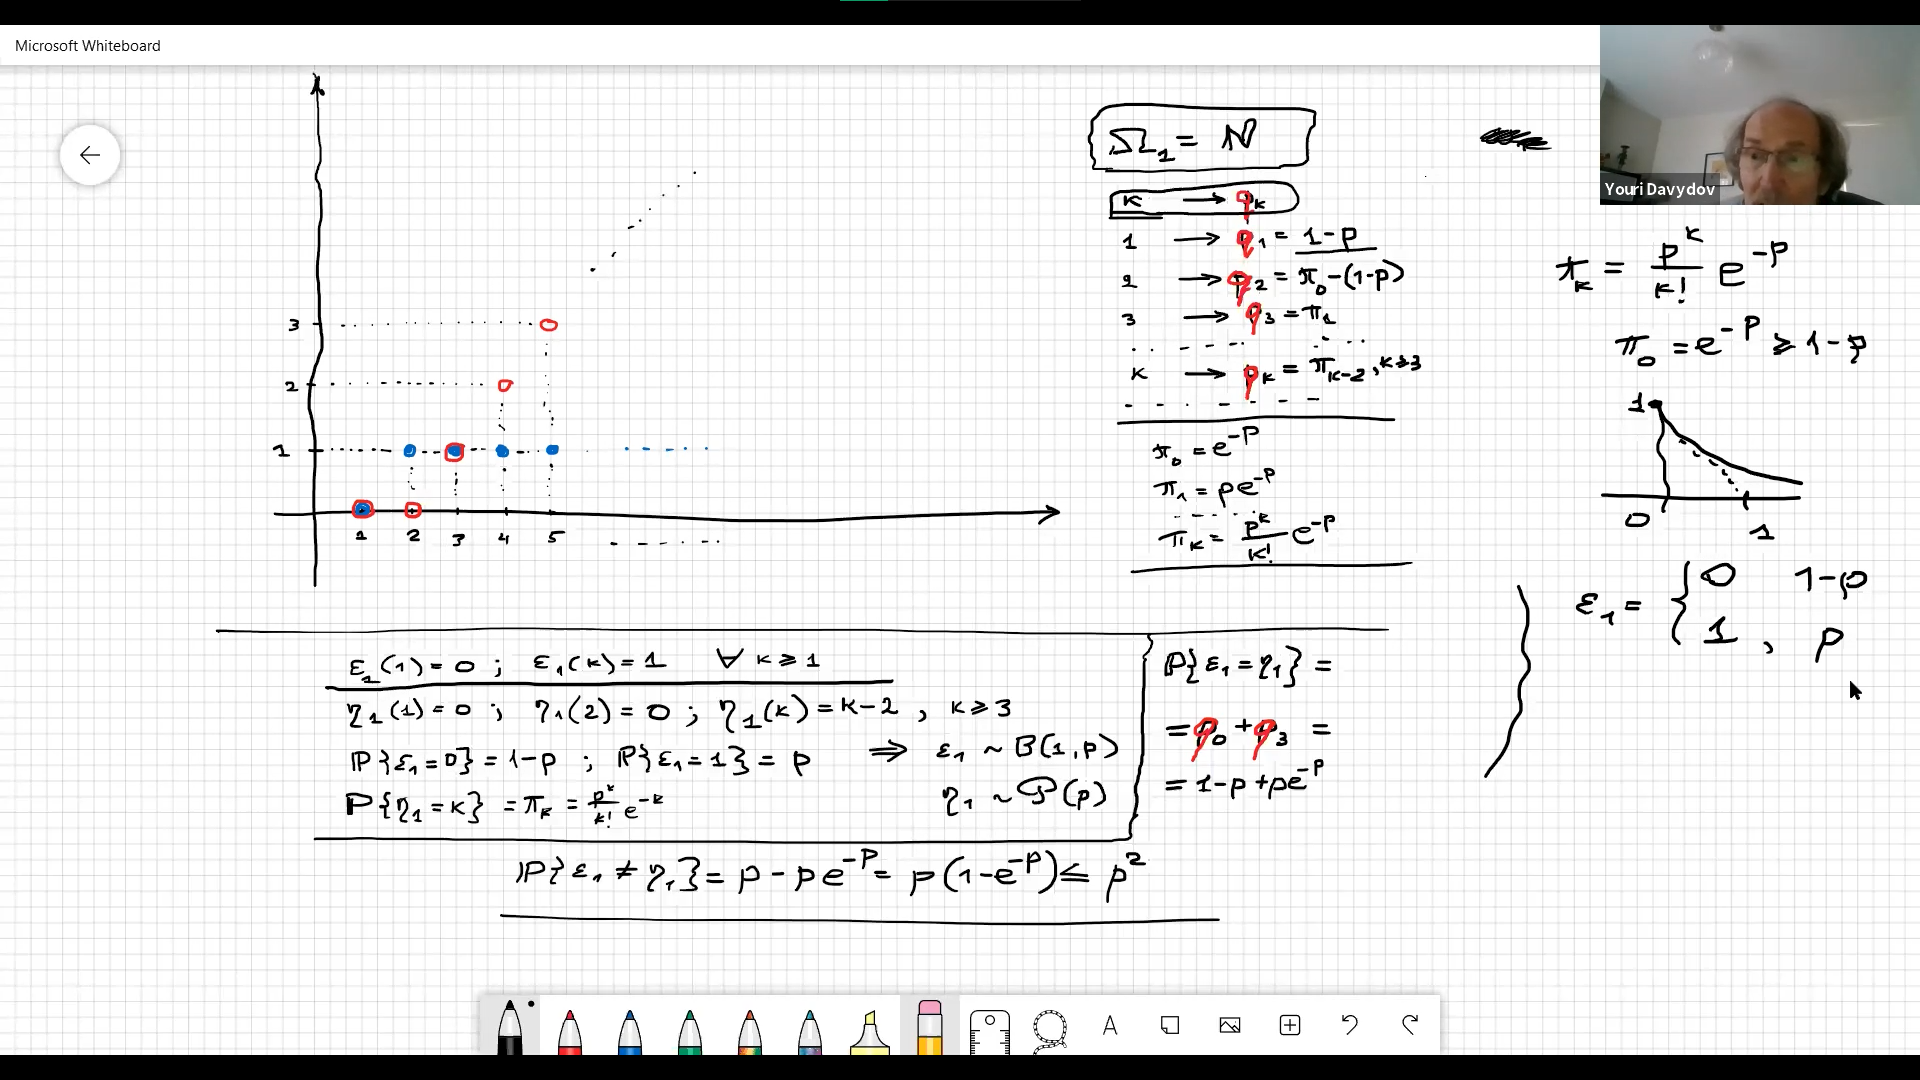
\includegraphics[width=\textwidth]{DPT-1.png}
            % \caption{Замена ручек лентами Мёбиуса}
            % \label{surface_typisation_picture_6}
            \todo[inline]{Перерисовать.}
        \end{figure}
        Несложно видеть, что
        \[\varepsilon_1 \sim B(1, p), \qquad \text{ а } \qquad \eta_1 \sim \mathcal{P}(p).\]
        При этом
        \[
            \PP_1\{\varepsilon_1 \neq \eta_1\}
            = 1 - \PP_1\{\varepsilon_1 = \eta_1\}
            = 1 - \PP_1(\{-1; 1\})
            = 1 - ((1-p) + p e^{-p})
            = p (1 - e^{-p})
            \leqslant p^2.
        \]

        Теперь сделаем ещё $n-1$ дубликатов нашего пространства и построенных случайных величин и перемножим их как в теореме \ref{probability-spaces-multiplication-theorem}. Получим пространство $(\Omega, \mathcal{F}, \PP)$ в котором выбраны случайные величины $\{\varepsilon_i\}_{i=1}^n$ и $\{\eta_i\}_{i=1}^n$, где
        \[\varepsilon_i \sim B(1, n), \qquad \text{ а } \qquad \eta_i \sim \mathcal{P}(p).\]
        При этом семейства $\{\varepsilon_i\}_{i=1}^n$ и $\{\eta_i\}_{i=1}^n$ независимы. Значит
        \[
            S_n \sim B(n, p) \sim X := \sum_{i=1}^n \varepsilon_i
            \qquad \text{ и } \qquad
            S \sim \mathcal{P}(np) \sim Y := \sum_{i=1}^n \eta_i.
        \]

        Следовательно
        \[
            \{X \neq Y\} \subseteq \bigcup_{i=1}^n \{\varepsilon_i \neq \eta_i\}
            \quad \Longrightarrow \quad
            \PP\{X \neq Y\} \leqslant \sum_{i=1}^n \PP\{\varepsilon_i \neq \eta_i\} \leqslant np^2.
        \]
        Отсюда имеем, что
        \begin{align*}
            |\PP\{S_n \in A\} - \PP\{S \in A\}|
            &= |\PP\{X \in A\} - \PP\{Y \in A\}|\\
            &= |\PP\{X \in A \wedge Y \notin A\} - \PP\{Y \in A \wedge X \notin A\}|\\
            &\leqslant \PP\{X \in A \wedge Y \notin A\} + \PP\{Y \in A \wedge X \notin A\}\\
            &\leqslant \PP\{X \neq Y\}\\
            &\leqslant np^2.
        \end{align*}
    \end{proof}

    \begin{corollary}
        Пусть дано $n \in \NN \cup \{0\}$ и случайные события $S_n \sim B(n, p)$ и $S \sim \mathcal{P}(np)$. Тогда
        \[\sum_{k=0}^\infty |\PP\{S_n = k\} - \PP\{S = k\}| \leqslant 2np^2.\] 
    \end{corollary}

    \begin{proof}
        Обозначим
        \[
            B_+ := \{k \mid \PP\{S_n = k\} \geqslant \PP\{S = k\}\}
            \qquad \text{ и } \qquad
            B_- := (\NN \cup \{0\}) \setminus B_+.
        \]
        Тогда понятно, что
        \begin{align*}
            \sum_{k=0}^\infty |\PP\{S_n = k\} - \PP\{S = k\}|
            &= \sum_{k \in B_+} (\PP\{S_n = k\} - \PP\{S = k\}) - \sum_{k \in B_-} (\PP\{S_n = k\} - \PP\{S = k\})\\
            &= (\PP\{S_n \in B_+\} - \PP\{S \in B_+\}) - (\PP\{S_n \in B_-\} - \PP\{S \in B_-\})\\
            &\leqslant |\PP\{S_n \in B_+\} - \PP\{S \in B_+\}| + |\PP\{S_n \in B_-\} - \PP\{S \in B_-\}|\\
            &\leqslant np^2 + np^2 = 2np^2
        \end{align*}
    \end{proof}


\end{document}